\documentclass{article}
% \usepackage{etex}
% if you need to pass options to natbib, use, e.g.:
% \PassOptionsToPackage{numbers, compress}{natbib}
% before loading nips_2016
%
% to avoid loading the natbib package, add option nonatbib:
% \usepackage[nonatbib]{nips_2016}

\usepackage[final]{nips_2016}

% to compile a camera-ready version, add the [final] option, e.g.:
% \usepackage[final]{nips_2016}

\usepackage[utf8]{inputenc} % allow utf-8 input
\usepackage[T1]{fontenc}    % use 8-bit T1 fonts
\usepackage{hyperref}       % hyperlinks
\usepackage{url}            % simple URL typesetting
\usepackage{booktabs}       % professional-quality tables
\usepackage{amsfonts}       % blackboard math symbols
\usepackage{nicefrac}       % compact symbols for 1/2, etc.
\usepackage{microtype}      % microtypography
\usepackage{graphicx}
\usepackage{listings}
\usepackage[thinlines]{easytable}
\usepackage{lipsum}
\usepackage{verbatim}
\usepackage{amsmath}
\usepackage[toc,page]{appendix}

\usepackage{adjustbox} % Turning a table 90 degrees
\usepackage{lscape} % Turning a page 90 degrees
\usepackage{rotating}

\usepackage{caption}
\usepackage{subcaption}

% Fixing space between text and section titles
\usepackage{titlesec}
\titlespacing\section{0pt}{14pt plus 4pt minus 2pt}{0pt plus 2pt minus 2pt}
\titlespacing\subsection{0pt}{12pt plus 4pt minus 2pt}{0pt plus 2pt minus 2pt}
\titlespacing\subsubsection{0pt}{10pt plus 4pt minus 2pt}{0pt plus 2pt minus 2pt}

% FIX titlesec bug which removed section numbering 
\usepackage{etoolbox}
\makeatletter
\patchcmd{\ttlh@hang}{\parindent\z@}{\parindent\z@\leavevmode}{}{}
\patchcmd{\ttlh@hang}{\noindent}{}{}{}
\makeatother

\usepackage{color}
\definecolor{deepblue}{rgb}{0,0,0.5}
\definecolor{deepred}{rgb}{0.6,0,0}
\definecolor{deepgreen}{rgb}{0,0.5,0}
\definecolor{mygreen}{rgb}{0,0.6,0}

\DeclareFixedFont{\ttb}{T1}{txtt}{bx}{n}{7} % for bold
\DeclareFixedFont{\ttm}{T1}{txtt}{m}{n}{7}  % for normal

\graphicspath{{/home/jensesi/projects/ITU_individual_project/report/v2/imgs/}}

\lstset{ 
otherkeywords={name, shape, dtype, initializer, value, filters, stride, padding},
breaklines=true,
tabsize=1,
language=Python,
basicstyle=\ttm,
commentstyle=\color{mygreen},
keywordstyle=\ttb\color{deepblue},
stringstyle=\color{deepgreen},
showstringspaces=false,
emphstyle=\ttb\color{deepred},
keepspaces=false
}  

\title{Object Detection: How Noise Patterns Affect the Performance of the Single Shot Multibox Detector}

% The \author macro works with any number of authors. There are two
% commands used to separate the names and addresses of multiple
% authors: \And and \AND.
%
% Using \And between authors leaves it to LaTeX to determine where to
% break the lines. Using \AND forces a line break at that point. So,
% if LaTeX puts 3 of 4 authors names on the first line, and the last
% on the second line, try using \AND instead of \And before the third
% author name.

\author{
  Simon B. Jensen\\
  Software Development \& Technology\\
  IT University of Copenhagen\\
  \texttt{sije@itu.dk} \\
  %% examples of more authors
  %% \And
  %% Coauthor \\
  %% Affiliation \\
  %% Address \\
  %% \texttt{email} \\
}

\begin{document}
% \nipsfinalcopy is no longer used

\maketitle

\section{Introduction}
\label{sec:introduction}
In the last few years object detection challenges such as the Pascal Visual Object Classes Challenge (Pascal VOC)\footnote{http://host.robots.ox.ac.uk/pascal/VOC/} and the ImageNet Large Scale Visual Recognition Competition (ILSVRC)\footnote{http://www.image-net.org/challenges/LSVRC/} have seen tremendous increases in detection performances due to new development in Deep Learning methods. More specifically development in Convolutional Neural Networks (CNNs) - a specific branch of Deep Learning. The performance of the top object detectors are now at a point where they have even surpassed human capabilities on these specific challenges. One could, however, argue that the images of these challenges are not realistic as the images are often ideally cropped, non-blurry and mostly only contain a few specific objects, for which the systems are optimized for. The human visual system is seemingly still superior when the settings are more realistic and non-ideal. 

We investigate whether this is actually the case, by asking the question: What happens to an object detector's performance if we add noise to the images before feeding them into the detector? Where the reason for adding noise to the images is to simulate a more realistic and non-ideal setting that e.g. also adverse weather scenarios, like rain-, snow- or foggy weather, could impose on a camera sensor. The effects could for instance be a blurred image or an incomplete image etc. Typically humans are able to deviate from these effects and are somehow still able to identify objects when the input is non-ideal. 

For this project we investigate how noise influence the detection performance of a state-of-the-art object detection systems, the Single Shot Multibox Detector (SSD) \citep{SSD}. We use an average filter and salt and pepper noise to simulate adverse weather scenarios. For testing and evaluating the object detection systems we utilize the Pascal VOC data set.  

\section{The Data: Pascal VOC}
The following section introduces and describes the Pascal VOC data set and, in short, it's role as a bench marking data set. The first part of the section can be skipped if the reader is already familiar with the data set.

There exists only a handful of image based data sets which are openly available to the public, and where the images and corresponding labels are both of high quality and there are a substantial amount of them. Thereby containing the key properties for serving as a valid benchmark data set. The Pascal VOC image data set is such a data set. Other such data sets are e.g. The ImageNet, COCO \footnote{http://cocodataset.org/\#home} and KITTI Vision \footnote{http://www.cvlibs.net/datasets/kitti/}. What is significant by publicly available benchmark data sets is the fact that they, in opposition to strictly private or company owned data sets, indulges to good competition between competing factions and can serve as a fair basis for comparison. Competition and the possibility for comparison will typically motivate and provoke even faster development in an area. And this is exactly what the Pascal VOC data set has done, since the first Pascal VOC challenge started in 2005, for the area of object detection among other computer vision challenges. It has since been held as a yearly competition, each year presenting new systems which pushed the boundaries for what is possible for computer vision systems. In this project we utilize the Pascal VOC data set for evaluation of the SSD object detection system. It should be noted that the Pascal VOC competition was last time held in 2012. But the evaluation server is still online and the data set can easily serve as a valid basis for the purpose of this project.  

\subsection{Pascal VOC and Object Detection}
In this project we focus on the object detection part of the Pascal VOC data set, as we are interested in testing the robustness of an object detector. But the Pascal VOC competition also consists of numerous other computer vision challenges, such as image classification, instance segmentation and more advanced challenges such as action classification. 

The object detection part of the challenge consists of a training-, validation- and test data set which consists of images with at least one, but possibly multiple objects in them. There are 20 different object classes which are shown, together with their quantities in the train-, validation- and test set, in table \ref{table:pascal-voc-classes}). As can be seen, the distribution of object classes in the data set is very uneven meaning that some object classes are much more frequent than others. The number of images in the data set is distributed as follows:
\begin{itemize}
	\setlength\itemsep{0.2em}
	\item Number of training images (Pascal VOC 2007 + Pascal VOC 2012): 8218
	\item Number of validation images (Pascal VOC 2007 + Pascal VOC 2012): 8333
	\item Number of test images (Pascal VOC 2007): 4952
\end{itemize}

The goal of the Pascal VOC object detection challenge is to detect both the correct object classes and locations of potentially multiple objects in an image. It should be noted that multiple objects from multiple classes may be present in the same image. The location of an object is simply represented by a 2D bounding box which surrounds the extent of the object visible in the image. When determining how well a object detector is performing the evaluation metric used is the mean Average Precision (mAP), which we explain in section \ref{sec:metrics}. The Pascal VOC images typically depict realistic scenes (see figure \ref{fig:pascal-voc-1} for examples). The data set consists of images crawled from flickr and from Microsoft Research Cambridge (MSRC) data set. For more information on the data set we refer to \url{http://host.robots.ox.ac.uk/pascal/VOC/#history}. 

\begin{table}[htp]
\small
\begin{minipage}{0.48\textwidth}
	\centering
    \begin{TAB}(r,0.3cm,0.5cm)[0.5pt]{|c|c|c|c|c|}{|c|c|c|c|c|c|c|c|c|c|c|}
    \textbf{Object class} & \textbf{Train (\#)} & \textbf{Val (\#)} & \textbf{Test (\#)} & \textbf{Total (\#)} \\
	aeroplane & 626 & 659 & 311 & 1596 \\
bicycle & 612 & 596 & 389 & 1597 \\
bird & 886 & 934 & 576 & 2396 \\
boat & 716 & 681 & 393 & 1790 \\
bottle & 1087 & 1029 & 657 & 2773 \\
bus & 448 & 461 & 254 & 1163 \\
Car & 2017 & 1991 & 1541 & 5549 \\
cat & 800 & 816 & 370 & 1986 \\
chair & 2183 & 2155 & 1374 & 5712 \\
cow & 540 & 518 & 329 & 1387 \\
    \end{TAB}
\end{minipage}\hfill % maximize space between the minipages
\begin{minipage}{0.48\textwidth}
	\centering
    \begin{TAB}(r,0.3cm,0.5cm)[0.5pt]{|c|c|c|c|c|}{|c|c|c|c|c|c|c|c|c|c|c|}
    \textbf{Object class} & \textbf{Train (\#)} & \textbf{Val (\#)} & \textbf{Test (\#)} & \textbf{Total (\#)} \\
	diningtable & 521 & 536 & 299 & 1356 \\
	dog & 1039 & 1040 & 530 & 2609 \\
	horse & 584 & 572 & 395 & 1551 \\
	motorbike & 568 & 573 & 369 & 1510 \\
	Pedestrian & 7724 & 7852 & 5227 & 20803 \\
	pottedplant & 862 & 862 & 592 & 2316 \\
	sheep & 700 & 647 & 311 & 1658 \\
	sofa & 617 & 594 & 396 & 1607 \\
	train & 485 & 499 & 302 & 1286 \\
	tvmonitor & 603 & 590 & 361 & 1554 \\
	\end{TAB}
\end{minipage}
\caption{\textit{The 20 Object classes of the Pascal VOC data set and their quantities in the 2007 + 2012 train- and validation data sets and the 2007 test data sets}}
\label{table:pascal-voc-classes}
\end{table} 

For this project we test the object detection system on both the original 4952 unmodified Pascal VOC test images, but also on the test images which have been blurred or which have added salt and pepper noise, as described in section \ref{sec:noise-patterns}. Thereby gaining knowledge about how robust the object detector is toward noise, which is suppose to simulate the effects adverse weather scenarios could impose on a camera sensor. We use pre-trained weights which have been trained using the entire combined Pascal VOC 2007 + 2012 training- and validation datasets but this is further described in subsection \ref{subsec:ssd-in-tensorflow}.

\begin{figure}
\begin{subfigure}{.5\linewidth}
\captionsetup{width=.9\linewidth}
\centering
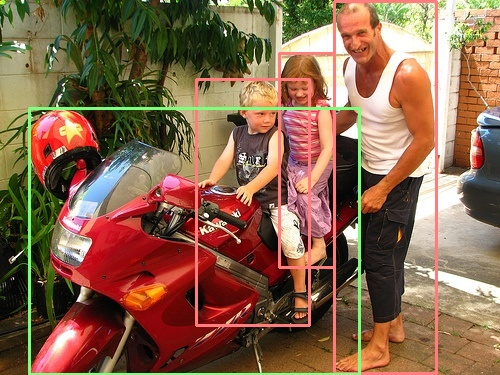
\includegraphics[scale=.3]{000058}
\caption{\textit{Image of three Person objects and a Motorbike object}}
\label{fig:pascal-voc-1.1}
\end{subfigure}%
\begin{subfigure}{.5\linewidth}
\captionsetup{width=.9\linewidth}
\centering
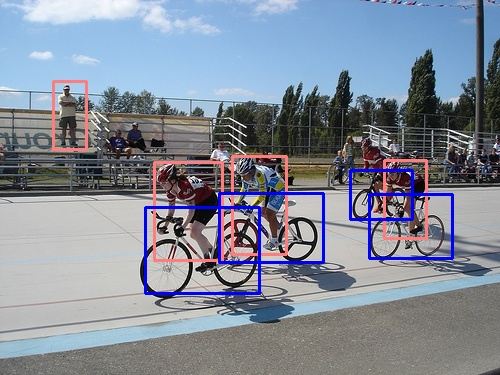
\includegraphics[scale=.3]{000527}
\caption{\textit{Image of four Bicycle objects and four Person objects}}
\label{fig:pascal-voc-1.2}
\end{subfigure}\\[1ex]
%\caption{\ref{fig:pascal-voc-1.1} Image of a bicycle and two persons from the Pascal VOC test dataset. \ref{fig:pascal-voc-1.2} Image of three airplanes from the Pascal VOC test dataset}
\caption{\textit{Images from the Pascal VOC test data set. 2D Bounding Boxes indicate the location and object class of the objects according to the ground-truth labels}}
\label{fig:pascal-voc-1}
\end{figure}

\section{Noise Patterns and Object Detection}
The following section argues why it is relevant to test an object detection systems on input images with added noise and further introduces the two noise patterns used in this project, blur by an average filter and salt and pepper noise.

\subsection{Motivation: Why does Noise on Images matter?}
Let us dwell upon the question of why we are interested in testing how object detection systems perform on images with added noise? Let us consider the case of a vehicle driving on a rainy day. The rainy weather makes the outside world look different, when seen through the car windows, from how it usually looks on a clear day. The traffic lights, the other cars in the traffic and the pedestrians has possibly become more blurry and unclear due to the water on the car window. 

When a human driver is sitting behind the steering wheel the rainy weather means it becomes harder for the driver to detect objects he or she sees through the car windows. But the human visual perception system is nevertheless able to deviate well enough from these changes so that we can navigate (more or less) safely in the traffic, even through adverse weather scenarios. Other weather circumstances could likewise change the looks of the world seen through the car windows. Consider snowy weather or foggy weather. Figure \ref{fig:car-in-rain} and \ref{fig:car-in-snow} show examples of how rain and snow can affect the world seen from inside the car. 

\begin{figure}[h]
\begin{subfigure}{.5\linewidth}
\captionsetup{width=.9\linewidth}
\centering
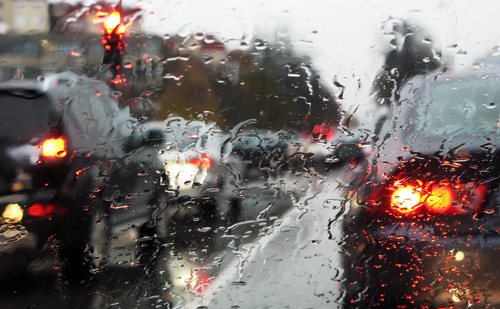
\includegraphics[scale=1.5]{car-in-rain}
\caption{\textit{Image of the possible effects of rain weather}}
\label{fig:car-in-rain}
\end{subfigure}%
\begin{subfigure}{.5\linewidth}
\captionsetup{width=.9\linewidth}
\centering
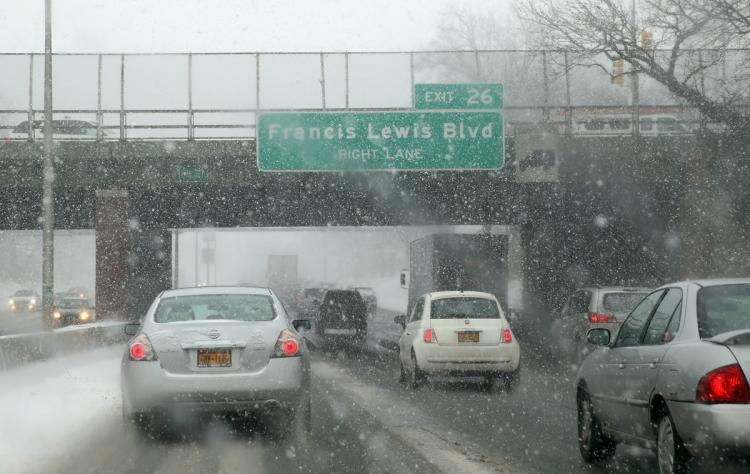
\includegraphics[scale=.24]{car-in-snow}
\caption{\textit{Image of the possible effects of snow weather}}
\label{fig:car-in-snow}
\end{subfigure}\\[1ex]
\caption{\textit{Examples of the possible effects adverse weather scenarios could impose on the vision from the inside of a car. A camera sensor, capturing input images to an object detector, could likely experience the same effects. Images were found by a simple Google search. Original image urls are: \url{http://www.carguide.ph/2016/08/driving-in-downpour-practical-rainy-day.html} and \url{http://www.nydailynews.com/news/national/snor-easter-blizzard-spares-new-york-city-article-1.2093191}}}
\label{fig:car-in-weathers}
\end{figure}

\subsection{Average Filtering Blur and Salt and Pepper Noise}
\label{sec:noise-patterns}
In order to simulate different real world adverse weather scenarios we apply blur by using an average filter and salt and pepper noise to the images. The blur is meant to simulate the impact rainy- or foggy weather could have on an camera sensor capturing input images. The salt and pepper noise is equally meant to simulate the impact rainy- or snowy weather could have on a camera sensor. We use kernels of size 7x7 and 9x9 for the average filtering blur. The effect of the blur can be seen in figure \ref{fig:dog2} and \ref{fig:dog3}. The average filtering blur is simply applied by sliding a kernel of a specific size (7x7 or 9x9 in our case) over the image pixels and averaging the pixel values.

We implemented the following simple Python function for applying the average filter blur, which requires the OpenCV and Numpy packages: 

\lstinputlisting[language=Python, firstline=1, lastline=5]{code/blur.py}
  
For the salt and pepper noise we implemented the following Python function which equally requires the Numpy package:

\lstinputlisting[language=Python, firstline=1, lastline=14]{code/salt-and-pepper.py}

The variable, \textbf{salt\_and\_pepper\_amount}, is set to $0.064$ for the first salt and pepper experiment and to $0.128$ in the second experiment. The effect of the salt and pepper noise can be seen in figure \ref{fig:dog4} and \ref{fig:dog5}. As mentioned, the noise should simulate the effect rainy-, snowy- or other adverse weather types could impose on a camera sensor. A comparison between the images in figure \ref{fig:car-in-weathers} and the images in figure \ref{fig:dogs} show that this assumption is not entirely far-fetched. 

\begin{figure}
\begin{subfigure}{\linewidth}
\centering
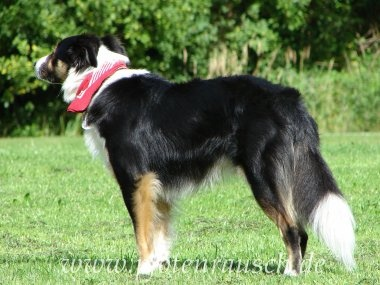
\includegraphics[scale=.3]{dog_(000018)}
\caption{\textit{The original untouched image}}
\label{fig:dog1}
\end{subfigure}
\begin{subfigure}{.5\linewidth}
\centering
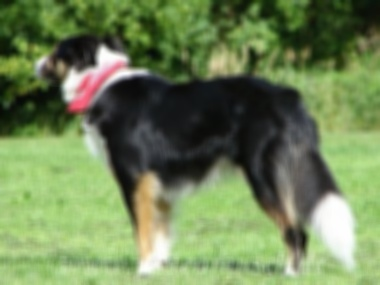
\includegraphics[scale=.3]{dog_gauss_7x7_(000018)}
\caption{\textit{Image blurred by a 7x7 average filter}}
\label{fig:dog2}
\end{subfigure}%
\begin{subfigure}{.5\linewidth}
\centering
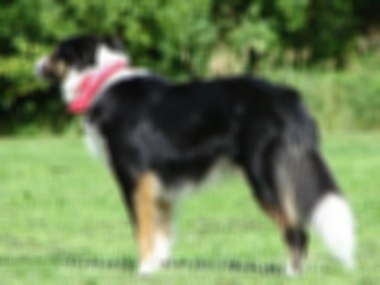
\includegraphics[scale=.3]{dog_gauss_9x9_(000018)}
\caption{\textit{Image blurred by a 9x9 average filter}}
\label{fig:dog3}
\end{subfigure}\\[1ex]
\begin{subfigure}{.5\linewidth}
\centering
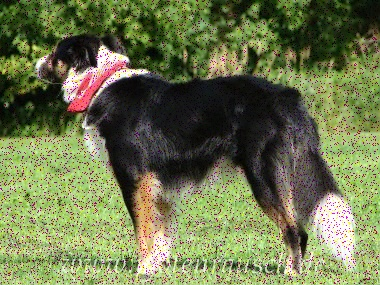
\includegraphics[scale=.3]{dog_sp_0064_(000018)}
\caption{\textit{Image with added salt and pepper noise}}
\label{fig:dog4}
\end{subfigure}%
\begin{subfigure}{.5\linewidth}
\centering
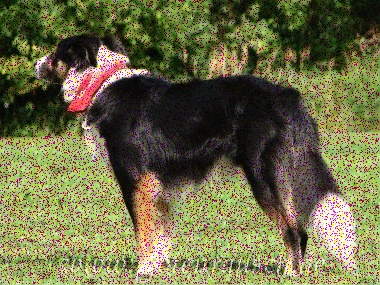
\includegraphics[scale=.3]{dog_sp_0128_(000018)}
\caption{\textit{Image with even more added salt and pepper noise}}
\label{fig:dog5}
\end{subfigure}\\[1ex]
\caption{\textit{Image (000018.jpg) of a dog from the Pascal VOC 2007 test set}}
\label{fig:dogs}
\end{figure}

\section{The Object Detector: Single Shot Multibox Detector (SSD)}
\label{sec:ssd}
The following section introduces and describes the CNN based object detection system, SSD \cite{SSD}, which is used and tested during the project. The system was, as of 2016, a state-of-the-art object detection systems, showing detection speeds faster than the YOLO network \cite{YOLO} while still obtaining prediction accuracy close to Faster R-CNN \cite{RCNN}. Still today, SSD and it's many derivatives are among the top performing object detectors. 
For this project we utilize a TensorFlow implementation of the SSD-300 network \footnote{https://github.com/balancap/SSD-Tensorflow}. In table \ref{table:ssd}, the ranking of the original SSD-300 and SSD-512 implementations on the Pascal VOC 2012 evaluation server can be seen. The distinction between SSD-300 and SSD-512 lies only on the size which the input image is scaled down/up to before it is fed to the network. Naturally, the SSD-300 is therefore a more lightweight edition of the SSD network than the SSD-512 and it is therefore also showing a slightly lower average prediction accuracy. 

\begin{center}
	\begin{table}[htp]
		\centering
    		\begin{TAB}(r,0.05cm,0.1cm)[2pt]{|c|c|c|c|c|c|}{|c|c|c|}
    			\textbf{Ranking} & \textbf{Name} & \textbf{mAP (\%)} & \textbf{max AP (\%)} & \textbf{min AP (\%)} & \textbf{submission date} \\
    			16 & SSD-512 & 82.2 & 93.9 (cat) & 60.9 (potted plant) & 10-Oct-2016 \\ 
    			27 & SSD-300 & 79.3 & 93.4 (cat) & 50.2 (potted plant) & 18-Oct-2016 \\ 
    		\end{TAB}
    		\caption{\textit{The original SSD-300 and SSD-512 implementations' ranking on the Pascal VOC 2012 evaluation server . SSD-300 and SSD-512 is ranking 27 and 16 respectively (as of 07.12.2017) with a mean average precision (mAP) of 79.3\% and 82.2\%. The results are found at: \url{http://host.robots.ox.ac.uk:8080/leaderboard/displaylb.php?challengeid=11&compid=4}}}
    		\label{table:ssd}
    \end{table}
\end{center}

%\begin{center}
%	\begin{table}[htp]
%		\centering
%    		\begin{TAB}(r,0.05cm,0.1cm)[2pt]{|c|c|c|c|c|c|}{|c|c|c|}
%    			\textbf{Ranking} & \textbf{Name} & \textbf{mAP (\%)} & \textbf{max AP (\%)} & \textbf{min AP (\%)} & \textbf{submission date} \\
%    			16 & SSD512 & 82.2 & 93.9 (cat) & 63.1 (bottle) & 10-Oct-2016 \\ 
%    			19 & YOLOv2 & 81.5 & 92.9 (cat) & 65.5 (bottle) & 21-Oct-2017 \\
%    		\end{TAB}
%    		\caption{The original SSD and YOLO (version 2) implementations' ranking on Pascal VOC 2012 test server. Ranking, respectively, 16 and 19 (as of 07.12.2017) with mean Average Precision (mAP) of 82.2\% and 81.5\%}
%    		\label{table:ssd}
%    \end{table}
%\end{center}

\subsection{The Backbone: VGG16}
Before going deeper into the SSD implementation it is worth first understanding it's \textbf{backbone}. By backbone we mean the CNN, which the images are fed into and which output good and useful feature maps for the object detection system to further work on. We assume that the reader is already familiar with CNNs and concepts such as convolutional- and pooling layers and the Rectified Linear Unit (ReLU) activation function. 
Most of today's successful object detection systems include one of the following popular standard CNNs in their architecture: The VGG-16 or VGG-19 (from University of Oxford)\cite{VGG}, Google's Inception models\cite{googlenet} or Microsoft's ResNets\cite{resnet}. 
Though the architectures of these CNNs are somewhat different they fundamentally do the same and they show only marginal difference in performance on classification tasks. What is great about them is the fact that they have been proven to have great classification performance on the ImageNet data set, thereby guaranteeing that the feature maps they output are of good quality, and it is possible to find and download pre-trained versions of them, which can save many days of training time. In this project we use the VGG-16 CNN as backbone, like the original SSD-300 implementation.  

What do these backbone CNNs then do that is so useful? As we mentioned the CNNs take images as input and output feature maps for the object detector to work with. The feature maps are maps of specific object features which the CNN has extracted from a given input image. The object features are extracted by passing the input image through a series of convolutional-, pooling- and activation layers. Where the weights of the convolutional layers have been learned during training. So basically the CNN, during training, have learned which features to look for in an input image and the feature maps are then the features which the CNN have extracted for a specific input image.   

\begin{figure}[h]
\centering
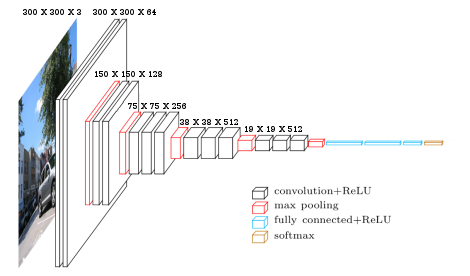
\includegraphics[scale=.55]{vgg16-2}
\caption{\textit{The original VGG-16 architecture (with dimensions modified for SSD-300). The last pooling layer, the three fully connected layers and the softmax layer are all excluded when VGG-16 is used as backbone CNN in the SSD network. The image originates from the original VGG paper \citep{VGG}}}
\label{fig:vgg16}     
\end{figure}    

For the original VGG-16 implementation the number of convolutional layers, which parameters are learned during training, are 13. The number 16 comes from the fact that VGG-16 actually includes 3 fully connected layers at it's end when it is used in classification tasks. However, the 3 fully connected layers are excluded when VGG is used as a backbone in the SSD network. Figure \ref{fig:vgg16} visualizes the VGG-16 architecture.

\subsection{Moving from Classification to Object Detection}
Now how do we move on from the SSD backbone, the VGG-16 CNN, which is able to perform classification tasks, to being able to perform object detection? What makes object detection such a complex task compared to classification is the fact that an image potentially contains multiple objects of interest, and for each of the objects both the class and localization in the image need to be determined.   
   
One of the ways SSD tackles this problem is by adding several feature layers of different scales to the end of the feature maps outputted by the VGG-16 CNN. For the SSD-300 model the number of added feature layers is 7 as can be seen in figure \ref{fig:SSD} (one is actually inside the VGG-16 body).   

\begin{figure}[h]
\centering
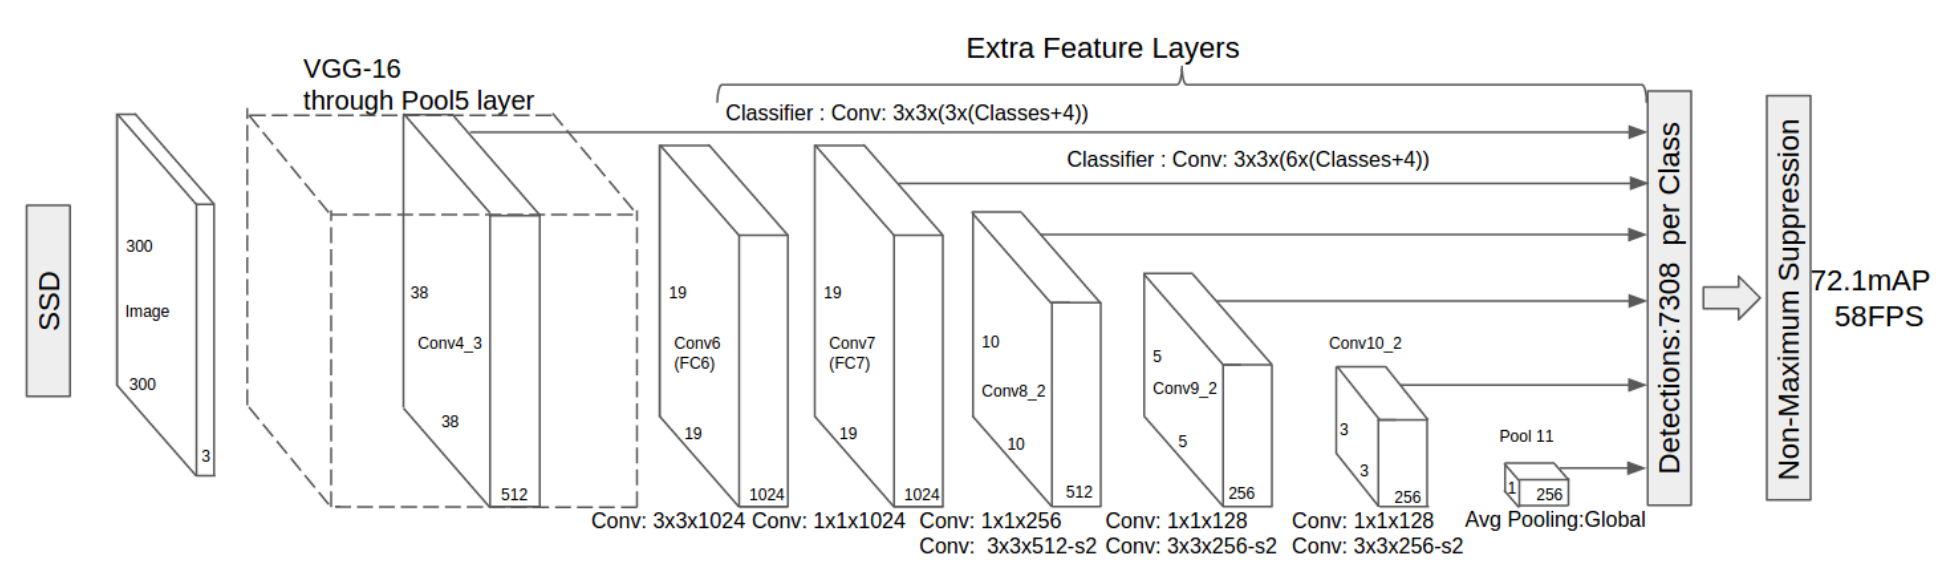
\includegraphics[scale=.34]{SSD}
\caption{\textit{The original SSD architecture. The image originates from the original SSD paper \citep{SSD}}}
\label{fig:SSD}     
\end{figure} 

The reason for adding feature layers of different scales is to be able to detect objects of many different sizes as the receptive fields, with respect to the input image, of each feature layer will be different. The feature layers are then discretized into a set of so called default boxes (equivalent to R-CNN's anchor boxes) of different aspect ratios and sizes and tried matched onto the feature layers. This procedure is best visualized with an image as can be seen in figure \ref{fig:ssd-feature-layer}

\begin{figure}[h]
\centering
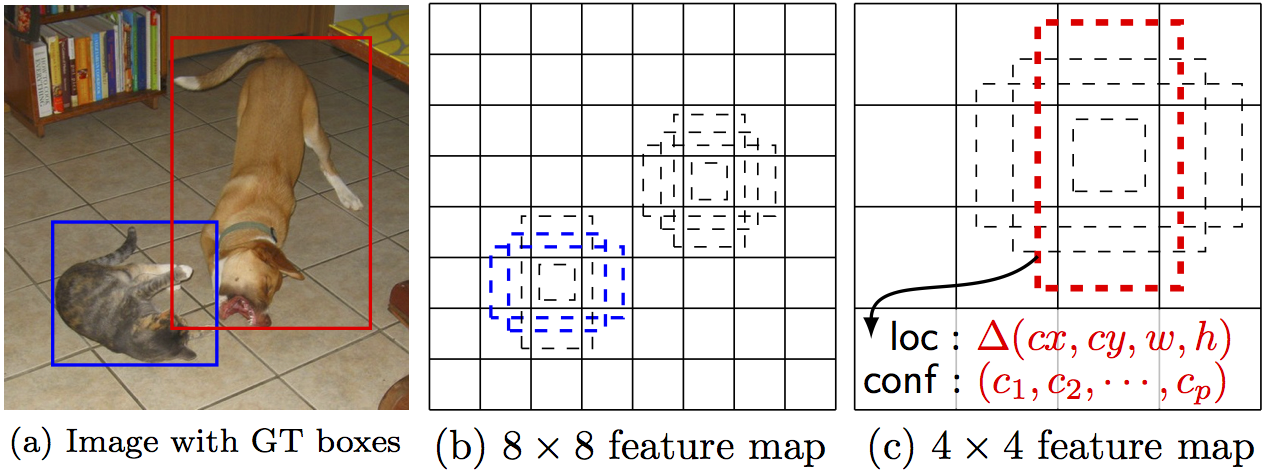
\includegraphics[scale=.8]{ssd-feature-layer}
\caption{\textit{The SSD evaluates a small set of default boxes of different aspect ratios at each location in several feature layers with different scales (e.g. 8x8 and 4x4 as seen in (b) and (c))}}
\label{fig:ssd-feature-layer}     
\end{figure}    

This approach to object detection has allowed actual real-time detection speeds. 
We refer to \cite{SSD} for further information on the approach and on the model loss function, which is a weighted sum between localization loss and confidence loss. 
 
\subsection{SSD in TensorFlow}
\label{subsec:ssd-in-tensorflow}
We use a TensorFlow implementation of the original SSD-300 network which can be found at \url{https://github.com/balancap/SSD-Tensorflow} and which has shown detection results equivalent to the original SSD implementation on the Pascal VOC 2007 test set. 
The implementation includes downloadable pre-trained weights for the SSD-300 model, trained on the entire Pascal VOC 2007 and 2012 training- and validation sets. The model works with data in the TFRecords file format\footnote{The TFRecords file format is a simple record-oriented binary format that many TensorFlow applications use for training data}, so in order to evaluate the SSD model, it is necessary to first convert the Pascal VOC datasets into TFRecords. We do that using the repository's included conversion script ``tf\_convert\_data.py'' and run the following command: 

\noindent
\begin{verbatim}
$ python tf_convert_data.py \
$ --dataset_name=pascalvoc \
$ --dataset_dir=[PATH to Pascal VOC]/ \ 
$ --output_name=voc_2007_test \
$ --output_dir=[PATH to store TFRecords]/
\end{verbatim}

In order to evaluate the model we use the repository's evaluation script: ``eval\_ssd\_network.py'' and run the following command:

\noindent
\begin{verbatim}
$ python eval_ssd_network.py \
$ --eval_dir=[PATH to store evaluation results and logs] \ 
$ --dataset_dir=[PATH to Pascal VOC TFRecords]/ \
$ --dataset_name=pascalvoc_2007 \ 
$ --dataset_split_name=test \ 
$ --model_name=ssd_300_vgg 
$ --checkpoint_path=[PATH to pretrained weights]/ssd_300_vgg.ckpt \
$ --batch_size=1
\end{verbatim}

We repeat this process for the Pascal VOC 2007 test data which has been blurred by an average filter as well as with added salt and pepper Noise and obtain the results shown in table \ref{table:ssd-performance}.

\begin{center}
	\begin{table}[htp]
		\centering
    		\begin{TAB}(r,0.05cm,0.1cm)[2pt]{|c|c|c|c|}{|c|c|c|c|c|c|}
    			\textbf{Input} & \textbf{mAP (\%)} & \textbf{max AP (\%)} & \textbf{min AP (\%)} \\
    			Original Images & 82.1 & 90.9 (cat) & 58.2 (bottle) \\ 
    			Avg. Filter (7x7) & 66.6 & 84.4 (cat) & 36.5 (bottle) \\ 
    			Avg. Filter (9x9) & 59.1 & 78.1 (cat) & 28.7 (bottle) \\ 
    			S\&P (0.064) & 71.9 & 88.0 (train) & 46.6 (bottle) \\ 
    			S\&P (0.128) & 65.8 & 81.2 (horse) & 34.9 (boat) \\ 
    		\end{TAB}
    		\caption{\textit{The performance of the SSD-300 TensorFlow implementation on the original untouched Pascal VOC 2007 test data set and on the Pascal VOC 2007 test data set modified by blur and salt and pepper noise}}
    		\label{table:ssd-performance}
    \end{table}
\end{center}

What we see in table \ref{table:ssd-performance} is that the SSD-300 TensorFlow implementation is achieving a mean average precision of 82.1 \% on the original unmodified Pascal VOC 2007 test data. This is a surprisingly high number, given that the model, according to the repository documentation, has only been trained on the Pascal VOC 2007 + 2012 training and validation data set. The performance even exceeds the performance of the original SSD-300 implementation. 
What we also see in the table is that the mean average precision, when an average filter with a kernel size of 9x9 is applied to test images, decrease from 82.1\% to 59.1\%. This is a relative decrease of ~28\%. In the case where salt and pepper noise is added to the test images, with the salt and pepper amount variable set to: $0.128$, the mean average precision decreases from 82.1\% to 65\%, which corresponds to a relative decrease of ~20\%. The entire evaluation results for each individual class is found in appendix \ref{sec:all-results} in table 5. The relative changes of each class can as well be found in the appendix in table 6. An interesting observation to note is that the two object classes, bus and train, have some of the lowest relative changes, even though the classes are among the quantitatively sparsest. A reason for this, could be the fact that both classes have very distinct features, e.g. the shape of the bus and train body. The pedestrian object class accounts for approximately one third of all the objects in the Pascal VOC data set but the decrease in performance is as high as for the bus and train object classes. The object classes with the biggest relative decreases are the bottle and boat classes, which deceases with ~49.9\% and ~50\%, respectively when the average filter blur (with kernel size 9x9) is applied to the test images. Another interesting observation here is to see that e.g. the average precision of the bottle class decreases much more drastically when blur is applied to the test images than when salt and pepper noise is added.

%\subsubsection{Statistics of Pascal VOC:}
%
%\textbf{Images in Pascal VOC:}
%
%
%\textbf{Objects Pascal VOC:}
%\begin{itemize}
%	\setlength\itemsep{0.2em}
%	\item Number of training objects (Pascal VOC 2007 + Pascal VOC 2012): 23618
%	\item Number of validation objects (Pascal VOC 2007 + Pascal VOC 2012): 23605
%	\item Number of test objects (Pascal VOC 2007): 14976
%\end{itemize}

\section{Precision/Recall and Mean Average Precision}
\label{sec:metrics}
A common metric used for evaluating object detection performance is the mean average precision (mAP). In order to understand the metric one first need to understand precision and recall. Precision and recall are given by the following equations:

\noindent\begin{minipage}{.5\linewidth}
\[\text{Precision}  = \frac{TP}{TP + FP}\]
\end{minipage}%
\begin{minipage}{.5\linewidth}
\[\text{Recall}  = \frac{TP}{TP + FN}\]
\end{minipage}

Where $\text{TP}$ stands for \textbf{true positive}, $\text{FP}$ stands for \textbf{false positive} and  $\text{FN}$ stands for \textbf{false negative}. A true positive, with respect to object detection, is the case where a predicted bounding box has an overlapping area with the ground-truth bounding box above a certain threshold value. The overlapping area is measured as the intersection over union (IoU):

\[\text{IoU} = \frac{\text{area}(B_{p} \cap B_{gt})}{\text{area}(B_{p} \cup B_{gt})} \]

For the Pascal VOC the IoU value has to be above 50\% for the predicted bounding box to count as a valid true positive. Figure \ref{fig:iou} shows an illustration of overlapping bounding boxes. The threshold value of 50\% is intentionally set this low, by the people behind Pascal VOC, to account for possible inaccuracies in the ground-truth bounding boxes. In a real world scenario where e.g. a vehicle navigates in the traffic the threshold value should likely be a lot higher, as not knowing the exact position of an object could potentially jeopardize lives.

A false positive, with respect to object detection, is when a non-object like e.g. the foreground/background or an object of another object class is predicted as being a specific object class. When evaluating the performance of Pascal VOC multiple predictions of the same object also count as false positives. If for instance the same object is predicted by 4 different bounding boxes only the first will count as a true positive the rest will count as false positives. Lastly, a false negative, with respect to object detection, is when no bounding box is predicted for the object of interest. 

There exists a inverse relationship (a trade-off) between the precision and recall values. So when one of them increases the other decreases. A precision/recall curve for each object class can be computed by changing a threshold value for which the detector dares to make predictions. The average precision is found by finding the value on the precision/recall curve where the sum of the precision and recall values are maximized. The mean average precision is simply taking the mean of the average precision found for each object class.    

\begin{figure}[h]
\centering
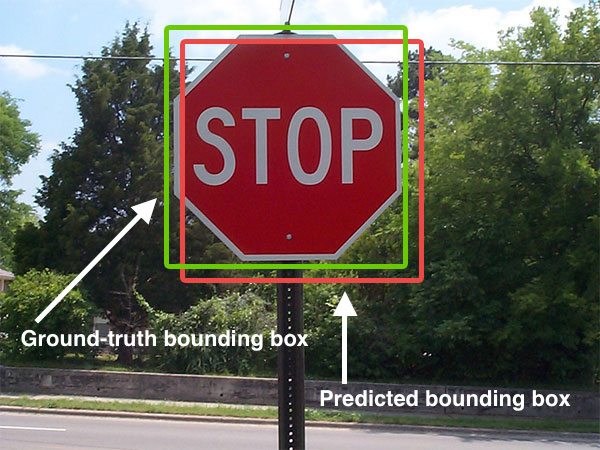
\includegraphics[scale=.35]{iou}
\caption{\textit{A predicted bounding box overlapping with a ground-truth bounding box. The image can be found at url: \url{https://www.pyimagesearch.com/2016/11/07/intersection-over-union-iou-for-object-detection/}}}
\label{fig:iou}     
\end{figure} 


\section{Perspectivation}
The result shown in table \ref{table:ssd-performance} shows that, when blur and salt and pepper noise is added to the Pascal VOC test images, the performance (measured in the mAP) of the SSD object detector decreases. This could also be the case for other object detecting systems. So it is worth asking, how we can deal with the challenges which the noise patterns impose on SSD and likely other object detectors. The following subsections present three approaches which could possibly enhance the robustness of the object detectors.   

\subsection{Generative Adversarial Neural Network}
One way that could possible increase the robustness of the object detector, towards noise, could be to pass input images through a Generative Adversarial Neural Network (GAN) before feeding them to a object detection systems. GANs are a special branch of artificial neural networks, which have been proven to be very effective when it comes to de-noising signals\cite{GAN}

\subsection{Image Augmentation}
Another possible approach could be to utilize the concept of image augmentation. Image augmentation is, like the name suggests, a way to augment the image data, such that it become more useful for a model performing a computer vision task. A data augmentation method, which SSD actually already utilizes, is for instance to extend the training set with copies or the original training data set, but adding color saturation to the copies. Another data augmentation method which SSD already utilizes is to extend the training data with images which zooms in on the objects marked by the ground-truth labels. There are a million other ways the training images could be augmented which could possibly increase the robustness of the object detector.  

\subsection{Sensor Fusion}
Another possible approach, which could make sense when the input data is served to the object detector by a camera sensor, is to increase the number of input sensors the model relies on. And further utilize fusion methods, such that if one sensor fails to deliver a good input image the model will rely on another sensor. In relation to this, a possible approach could be to extend the model to rely on a fused signal from multiple different types of sensors. e.g LIDAR data, radar, GPS and/or gated cameras. 


%\begin{TAB}(r,1cm,2cm)[5pt]{|c|c|}{|c|c|c|}% (rows,min,max)[tabcolsep]{columns}{rows}
%hi & tall one    \\
%hi & medium one  \\
%hi & standard one\\
%\end{TAB}

% STYLE
%The style files for NIPS and other conference information are
%available on the World Wide Web at
%\begin{center}
%  \url{http://www.nips.cc/}
%\end{center}

% LINKS
%\begin{center}
%  \url{https://google.com/protein+secondary+structure/}
%\end{center}
% PARAGRAPHS
%\paragraph{Paragraphs}
%
%There is also a \verb+\paragraph+ command available, which sets the
%heading in bold, flush left, and inline with the text, with the
%heading followed by 1\,em of space.


% CITATIONS
%
%The \verb+natbib+ package will be loaded for you by default.
%Citations may be author/year or numeric, as long as you maintain
%internal consistency. 
%
%The command \verb+\citet+, which produces citations
%appropriate for use in inline text.  For example,
%\begin{verbatim}
%   \citet{hasselmo} investigated\dots
%\end{verbatim}
%produces
%\begin{quote}
%  Hasselmo, et al.\ (1995) investigated\dots
%\end{quote}

%FOOTNOTES
%Footnotes should be used sparingly. 
%\footnote{Sample of the first footnote.} in the text. 


% FIGURES
%\begin{figure}[h]
%  \centering
%  \fbox{\rule[-.5cm]{0cm}{4cm} \rule[-.5cm]{4cm}{0cm}}
%  \caption{Sample figure caption.}
%\end{figure}


% TABLES
%We strongly suggest the use of the \verb+booktabs+ package,
%which allows for typesetting high-quality, professional tables:
%\begin{center}
%  \url{https://www.ctan.org/pkg/booktabs}
%\end{center}
%This package was used to typeset Table~\ref{sample-table}.
%
%\begin{table}[t]
%  \caption{Sample table title}
%  \label{sample-table}
%  \centering
%  \begin{tabular}{lll}
%    \toprule
%    \multicolumn{2}{c}{Part}                   \\
%    \cmidrule{1-2}
%    Name     & Description     & Size ($\mu$m) \\
%    \midrule
%    Dendrite & Input terminal  & $\sim$100     \\
%    Axon     & Output terminal & $\sim$10      \\
%    Soma     & Cell body       & up to $10^6$  \\
%    \bottomrule
%  \end{tabular}
%\end{table}

%Use unnumbered first-level heading for the references. Any choice of citation 
%style is acceptableas long as you are consistent. 
%\medskip

% References
\bibliographystyle{plain}
\bibliography{references}

\clearpage

\begin{appendices}
\section{SSD-300's Mean Average Precision on Pascal VOC}
\label{sec:all-results}
\begin{sidewaystable}[!htbp]
\captionsetup{width=.8\linewidth}
\centering
    \begin{TAB}(r,0.2cm,0.2cm)[.5pt]{|c|c|c|c|c|c|c|c|c|c|c|c|c|c|c|c|c|c|c|c|c|c|}{|c|c|c|c|c|c|}
   		\rotatebox{60}{\textbf{Input}} & \rotatebox{60}{\textbf{mAP}} & \rotatebox{60}{\textbf{aeroplane}} & \rotatebox{60}{\textbf{bicycle}} & \rotatebox{60}{\textbf{bird}} & \rotatebox{60}{\textbf{boat}} & \rotatebox{60}{\textbf{bottle}} & \rotatebox{60}{\textbf{bus}} & \rotatebox{60}{\textbf{Car}} & \rotatebox{60}{\textbf{cat}} & \rotatebox{60}{\textbf{chair}} & \rotatebox{60}{\textbf{cow}} & \rotatebox{60}{\textbf{diningtable}} & \rotatebox{60}{\textbf{dog}} & \rotatebox{60}{\textbf{horse}} & \rotatebox{60}{\textbf{motorbike}} & \rotatebox{60}{\textbf{Pedestrian}} & \rotatebox{60}{\textbf{pottedplant}} & \rotatebox{60}{\textbf{sheep}} & \rotatebox{60}{\textbf{sofa}} & \rotatebox{60}{\textbf{train}} & \rotatebox{60}{\textbf{tvmonitor}} \\
	Original & 82.1 & 	88.3 & 	83.3 & 	80.7 & 	72.7 & 	58.2 & 	88.7 & 	84.8 & 	90.9 & 	68.4 & 	87.1 & 	78.8 & 	90.7 & 	89.8 & 	87.8 & 	82.8 & 	67.1 & 	80.1 & 	86.7 & 	90.3 & 	85 \\ 
    7x7 & 66.6 & 	71 & 	72.4 & 	59.2 & 	46.6 & 	36.5 & 	74.8 & 	68.4 & 	84.4 & 	47.2 & 	68.4 & 	65.8 & 	81.9 & 	78.8 & 	77.6 & 	70 & 	46 & 	60.5 & 	73.8 & 	82.6 & 	66.2 \\
    9x9 & 59.1 & 	62.2 & 	65.4 & 	49.9 & 	36.4 & 	28.7 & 	70.1 & 	62.6 & 	78.1 & 	38.6 & 	57.5 & 	59.1 & 	73.4 & 	73.8 & 	72 & 	64.6 & 	38.5 & 	51.4 & 	66.4 & 	74.2 & 	59.7 \\
	S\&P 1 & 71.9 & 	62.3 & 	78.9 & 	64.9 & 	47.3 & 	46.6 & 	82.2 & 	76.6 & 	85.7 & 	58.8 & 	77.8 & 	73.1 & 	82.9 & 	84.7 & 	81.4 & 	77.1 & 	54.3 & 	64.8 & 	76.5 & 	88 & 73.8 \\
 	S\&P 2 & 65.8 & 	53.6 & 	76.2 & 	54.1 & 	34.9 & 	41.9 & 	76.1 & 	70.6 & 	80 & 	53.7 & 	70.1 & 	69.7 & 	77.5 & 	81.2 & 	77.2 & 	73.1 & 	49.5 & 	60.4 & 	69.8 & 	79.9 & 	67.5

    %Avg. Filter (9x9) & 59.13 & 78.1 (cat) & 28.7 (bottle) \\ 
    %S\&P (0.064) & 71.87 & 88.0 (train) & 46.6 (bottle) \\ 
    %S\&P (0.128) & 65.84 & 81.2 (horse) & 34.9 (boat) \\ 
    \end{TAB}
\label{table:results}
\caption{The average precision of each class when evaluating the TensorFlow implementation of the Single Shot Multibox Detetor (SSD-300) on the original unmodified Pascal VOC test data set, on the Pascal VOC test data with added blur (using average filtering with different kernel sizes) and on the Pascal VOC test data  with added salt and pepper noise}
\end{sidewaystable}

\begin{sidewaystable}[!htbp]
\captionsetup{width=.8\linewidth}
\centering
    \begin{TAB}(r,0.2cm,0.2cm)[.5pt]{|c|c|c|c|c|c|c|c|c|c|c|c|c|c|c|c|c|c|c|c|c|c|}{|c|c|c|c|c|}
   		\rotatebox{60}{\textbf{Input}} & \rotatebox{60}{\textbf{mAP}} & \rotatebox{60}{\textbf{aeroplane}} & \rotatebox{60}{\textbf{bicycle}} & \rotatebox{60}{\textbf{bird}} & \rotatebox{60}{\textbf{boat}} & \rotatebox{60}{\textbf{bottle}} & \rotatebox{60}{\textbf{bus}} & \rotatebox{60}{\textbf{Car}} & \rotatebox{60}{\textbf{cat}} & \rotatebox{60}{\textbf{chair}} & \rotatebox{60}{\textbf{cow}} & \rotatebox{60}{\textbf{diningtable}} & \rotatebox{60}{\textbf{dog}} & \rotatebox{60}{\textbf{horse}} & \rotatebox{60}{\textbf{motorbike}} & \rotatebox{60}{\textbf{Pedestrian}} & \rotatebox{60}{\textbf{pottedplant}} & \rotatebox{60}{\textbf{sheep}} & \rotatebox{60}{\textbf{sofa}} & \rotatebox{60}{\textbf{train}} & \rotatebox{60}{\textbf{tvmonitor}} \\
	7x7 & -18.9 & 	-19.6 & 	-13.1 & 	-26.7 & 	-35.9 & 	-37.2 & 	-15.7 & 	-19.3 & 	-7.2 & 	-31 & 	-21.5 & 	-16.5 & 	-9.7 & 	-12.3 & 	-11.7 & 	-15.5 & 	-31.4 & 	-24.5 & 	-14.9 & 	-8.6 & 	-22.1 \\
	9x9 & -28 & 	-29.5 & 	-21.5 & 	-38.2 & 	-49.9 & 	-50.7 & 	-21 & 	-26.2 & 	-14.1 & 	-43.6 & 	-34 & 	-25 & 	-19 & 	-17.8 & 	-18 & 	-22 & 	-42.6 & 	-35.8 & 	-23.4 & 	-17.9 & 	-29.8 \\
 S\&P 1 & -12.5 & 	-29.4 & 	-5.3 & 	-19.6 & 	-34.9 & 	-19.8 & 	-7.4 & 	-9.6 & 	-5.7 & 	-13.9 & 	-10.7 & 	-7.2 & 	-8.6 & 	-5.7 & 	-7.4 & 	-6.9 & 	-19.1 & 	-19.2 & 	-11.8 & 	-2.6 & 	-13.2 \\
 S\&P 2 & -19.8 & 	-39.3 & 	-8.5 & 	-33 & 	-52 & 	-27.9 & 	-14.3 & 	-16.7 & 	-12 & 	-21.5 & 	-19.6 & 	-11.5 & 	-14.5 & 	-9.6 & 	-12.1 & -11.7 & 	-26.1 & 	-24.6 & 	-19.5 & 	-11.6 & 	-20.6

    \end{TAB}
\label{table:relative-change}
\caption{The table shows the relative change of the mean average precision obtained by the SSD-300 TensorFlow implementation, when noise is added to the Pascal VOC test images, compared to mean average precision obtained on the unmodified test images. In all cases the relative change is, not surprisingly,  negative, which is marked with a negation sign}
\end{sidewaystable}

\end{appendices}
%\begin{adjustbox}{angle=90}
%\centering
%    \begin{TAB}(r,0.3cm,0.5cm)[0.5pt]{|c|c|c|c|c|c|c|c|c|c|c|c|c|}{|c|c|c|}
%   		\textbf{Input} & \textbf{mAP} & \textbf{aeroplane} & \textbf{bicycle} & \textbf{bird} & \textbf{boat} & \textbf{bottle} & \textbf{bus} & \textbf{Car} & \textbf{cat} & \textbf{chair} & \textbf{cow} & ... \\
%	Original & 82.11 & 88.25 & 83.28 & 80.7 & 72.68 & 58.16 & 88.74 & 84.77 & 90.88 & 68.36 & 87.13 & ...\\ 
%    Avg. Filter (7x7) & 66.6 & 70.97 & 72.35 & 59.19 & 46.61 & 36.54 & 74.77 & 68.41 & 84.37 & 47.16 & 68.4 & ...\\
%    %Avg. Filter (9x9) & 59.13 & 78.1 (cat) & 28.7 (bottle) \\ 
%    %S\&P (0.064) & 71.87 & 88.0 (train) & 46.6 (bottle) \\ 
%    %S\&P (0.128) & 65.84 & 81.2 (horse) & 34.9 (boat) \\ 
%    \end{TAB}
%\label{table:pascal-voc-classes}
%\end{adjustbox}

%\hspace{2em}
%
%\centering
%    \begin{TAB}(r,0.5cm,0.7cm)[0.5pt]{|c|c|c|c|c|c|c|c|c|c|c|c|c|}{|c|c|c|}
%   		\textbf{...} & \textbf{diningtable} & \textbf{dog} & \textbf{horse} & \textbf{motorbike} & \textbf{Pedestrian} & \textbf{pottedplant} & \textbf{sheep} & \textbf{sofa} & \textbf{train} & \textbf{tvmonitor} & \textbf{Max AP} & \textbf{Min AP}  \\
%	... & 78.81 & 90.7 & 89.81 & 87.84 & 82.78 & 67.06 & 80.13 & 86.72 & 90.34 & 85 & 90.88 & 58.16 \\ 
%    ... & 65.78 & 81.9 & 78.78 & 77.59 & 69.96 & 46.03 & 60.5 & 73.84 & 82.6 &	66.2 & 84.37 & 36.54 \\
%    %Avg. Filter (9x9) & 59.13 & 78.1 (cat) & 28.7 (bottle) \\ 
%    %S\&P (0.064) & 71.87 & 88.0 (train) & 46.6 (bottle) \\ 
%    %S\&P (0.128) & 65.84 & 81.2 (horse) & 34.9 (boat) \\ 
%    \end{TAB}
%\label{table:pascal-voc-classes}

\end{document}
